\documentclass{if-beamer}
\begin{document}
	
	\title[Campus Formoso do Araguaia]{Configuração de Redes e Servidores}
	\subtitle{Aula 4 }
	\author{Gilmar Gomes do Nascimento}
	\institute[IFTO]{
		Instituto Federal do Tocantins\\
		Campus Formoso do Araguaia
	}
	\date{\today}
	\logo{
		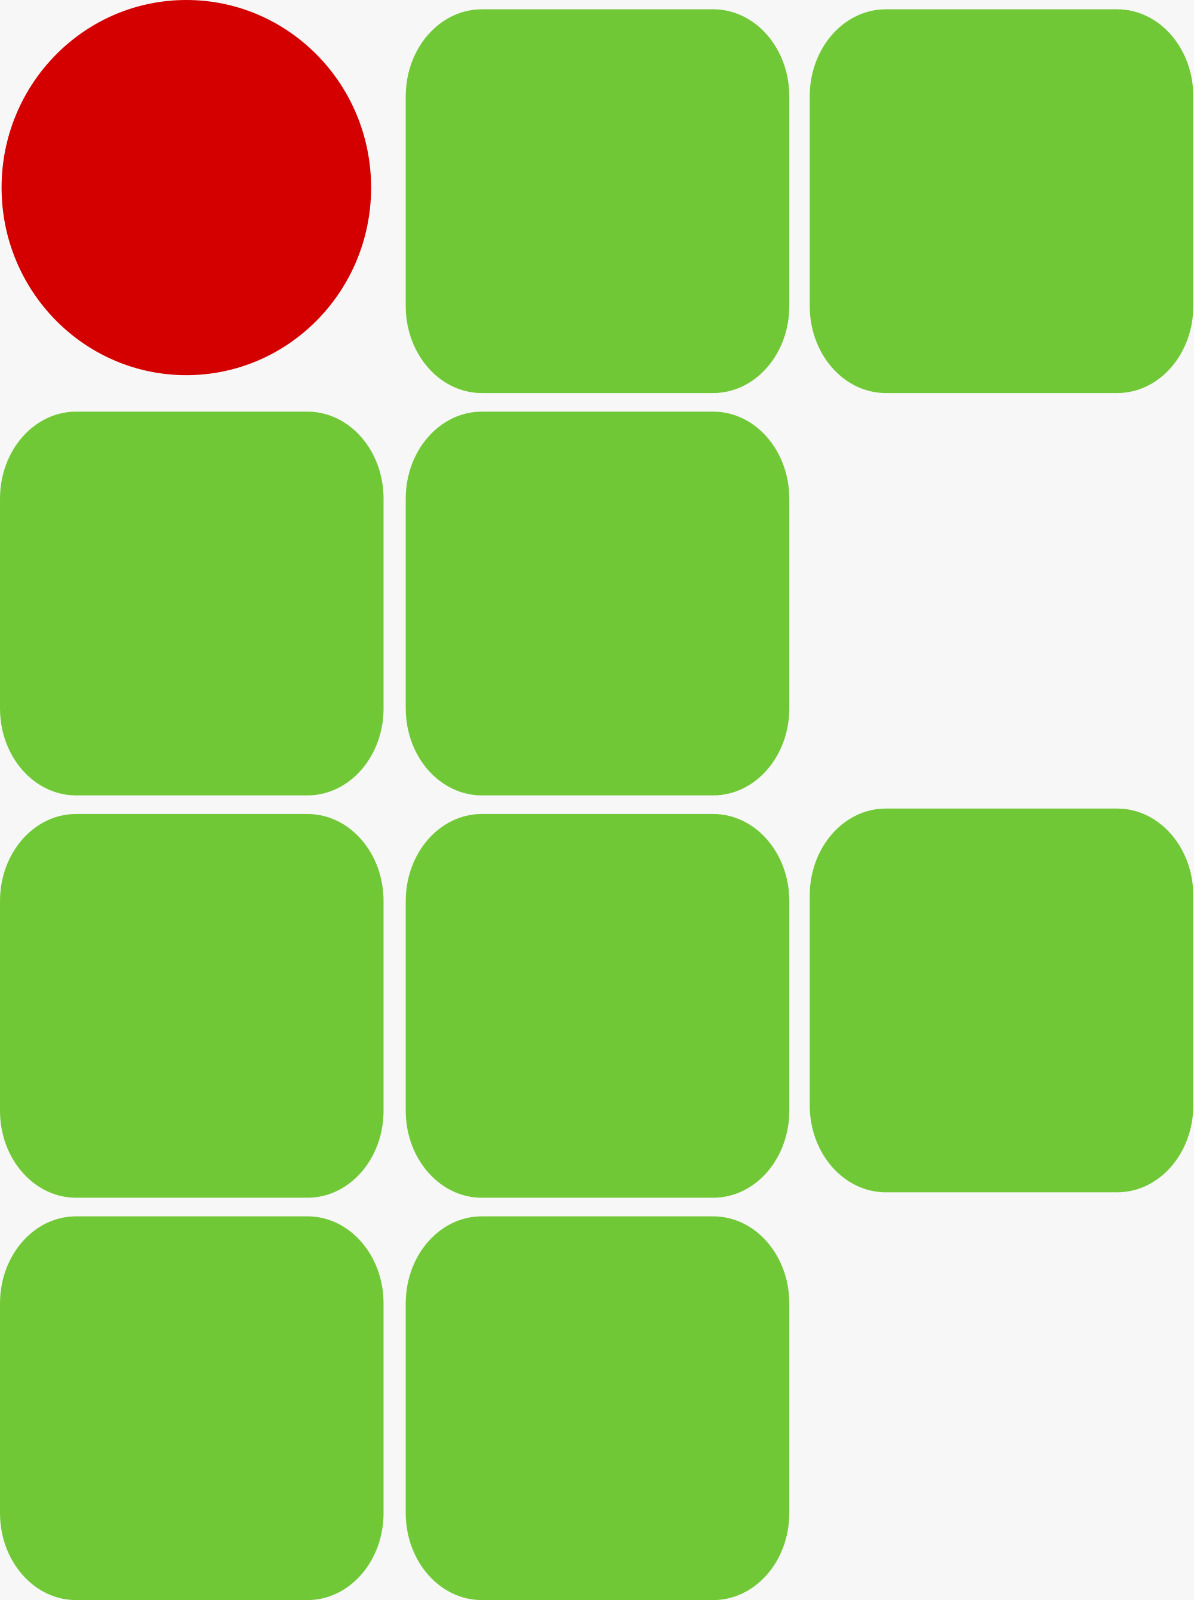
\includegraphics[scale=0.0085]{logo.jpg}
	}
	\subject{Servers} % metadata
	
	\graphicspath{{figuras/}}
	%---------------------------------------------------------------------------------
	
	\begin{frame}
		\titlepage
	\end{frame}

\begin{frame}{NGINX}
        \begin{figure}
           
\includegraphics[scale=0.35]{nginx.jpeg}
        \end{figure}
    \end{frame}   

    \begin{frame}{Nginx}

        \begin{quote}
            nginx (``engine x") is an HTTP web server, reverse proxy, content cache, load balancer, TCP/UDP proxy server, and mail proxy server. Originally written by Igor Sysoev and distributed under the 2-clause BSD License. Enterprise distributions, commercial support and training are available from F5, Inc.
        \end{quote}
        \begin{block}{Em português}
        O Nginx é um servidor web HTTP, proxy reverso, cache de conteúdo, balanceador de carga, proxy TCP/UDP e servidor de proxy de e-mail.
    \end{block}
  \end{frame}
%    \framebreak
%
        \begin{frame}{Pré-requisitos}
            \texttt{sudo apt install curl gnupg2 ca-certificates lsb-release debian-archive-keyring -y} 
        \end{frame}
        
        \begin{frame}[fragile]{Instalação do Nginx}
        	\begin{lstlisting}[language=bash]
sudo apt update
sudo apt install nginx -y
\end{lstlisting}
   \end{frame}
        
        \begin{frame}{Onde buscar informação oficial}
    \centering
    \Huge
    \texttt{nginx.org}
    
    \vspace{1cm}
    \Large
    \texttt{nginx.org/en/docs/}
    
    \vspace{1cm}
    \normalsize
    (documentação oficial)
\end{frame}

      \begin{frame}{Bem-vindo}
        	\begin{figure}
        		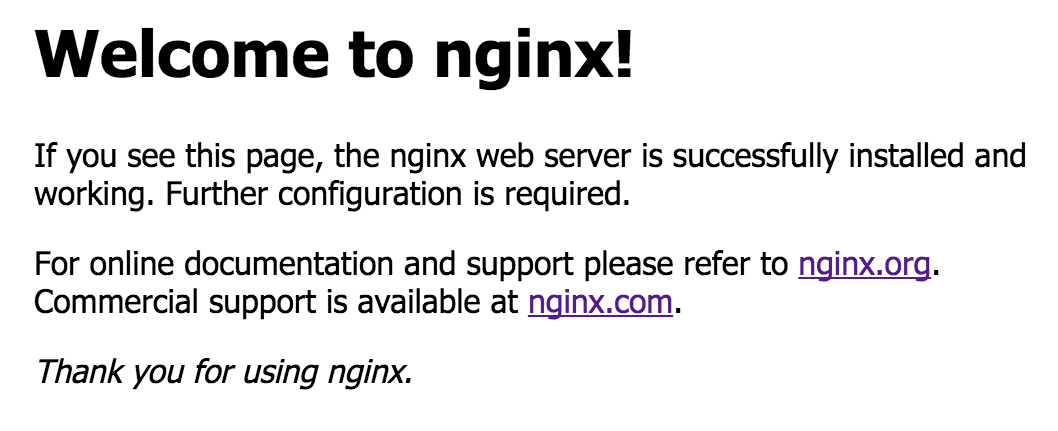
\includegraphics[scale=0.6]{welcome}
        	\end{figure}        
        \end{frame}
        
        \begin{frame}{Serviços}
        \begin{itemize}
        	\item Status
        	\item Start
        	\item Stop
        	\item Restart
        	\item Reload
        \end{itemize}        
        \end{frame}
        
        \begin{frame}{Nginx}
        \begin{itemize}
        	\item Qual porta?
        	\item Página ``inicial" do Ngnix 
        	\item Diretório dos arquivos
        \end{itemize}        
        \end{frame}
        
        \begin{frame}{Site estático x dinâmico}
    \begin{columns}
        \begin{column}{0.5\textwidth}
            \begin{block}{Estático}
                \begin{itemize}
                    \item HTML, CSS, imagens
                    \item Mesmo conteúdo para todos
                    \item Nginx entrega direto
                    \item Ex: \texttt{ola.html}
                \end{itemize}
            \end{block}
        \end{column}
        \begin{column}{0.5\textwidth}
            \begin{block}{Dinâmico}
                \begin{itemize}
                    \item PHP, Python, Node.js
                    \item Conteúdo muda por usuário
                    \item Precisa de servidor de aplicação
                    \item Ex: \texttt{login.php}
                \end{itemize}
            \end{block}
        \end{column}
    \end{columns}
   
\end{frame}

        \begin{frame}[fragile]{Permissões de leitura e escrita}
    O Nginx roda como usuário \texttt{www-data}. Os arquivos precisam ser legíveis por ele.
    
    
    \begin{lstlisting}[language=bash]
# Ver o dono dos arquivos
ls -la /var/www/html/

# Mudar o dono para www-data
sudo chown -R www-data:www-data /var/www/html/

# Permissões: dono le/escreve, grupo le, outros leem
sudo chmod -R 755 /var/www/html/
    \end{lstlisting}
    
  
\end{frame}
 \begin{frame}
   \begin{alertblock}{Atenção}
        Se o arquivo não for legível pelo \texttt{www-data}, o Nginx retorna erro \textbf{403 Forbidden}.
    \end{alertblock}
 \end{frame}
		
		\begin{frame}{LEMP}
			
\includegraphics[scale=0.2]{lemp.jpg}
		\end{frame}				
		
		\begin{frame}{PHP}
			\begin{figure}
				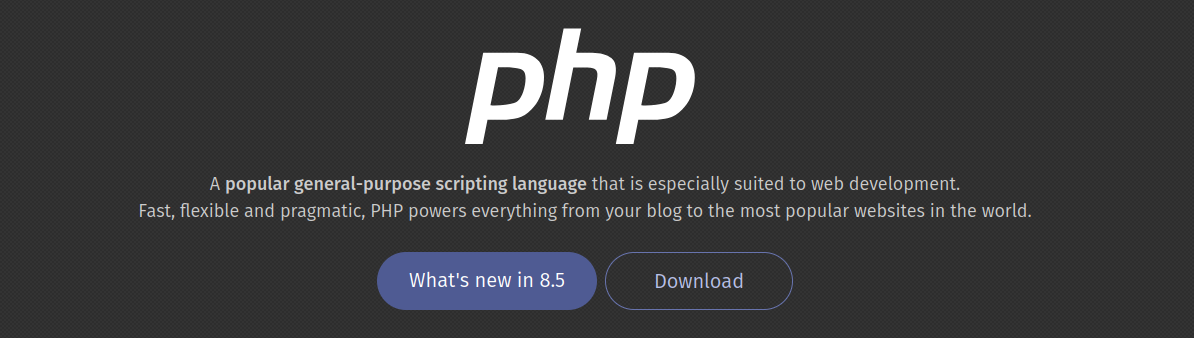
\includegraphics[scale=0.34]{php}
			\end{figure}
		\end{frame}
		
		\begin{frame}[fragile]{Instalar o PHP-FPM}
    		O PHP-FPM interpreta o código PHP.
    
    		\begin{lstlisting}[language=bash]
sudo apt update
sudo apt install php-fpm -y
\end{lstlisting}
    	\end{frame}
    	
    	\begin{frame}{Crie um arquivo em php}
    		\begin{itemize}
    			\item Salve com o nome: idade.php
    			\item Pergunte o ano que nasceu
    			\item Mostre a idade
    		\end{itemize}
    	\end{frame}
    	
    	\begin{frame}{No navegador}
    		\begin{itemize}
    			\item Teste a página criada inserindo informações
    	\end{itemize}    	
    	\end{frame}
    
% ============================================================
% REFERÊNCIAS
% ============================================================

%\begin{frame}[allowframebreaks]{Referências}
%	\begin{thebibliography}{9}
%		
%		\bibitem{cloudflare}
%		Cloudflare	\textit{O que é DNS? | Como o DNS funciona}. Disponível em: \url{https://www.cloudflare.com/pt-br/learning/dns/what-is-dns/}. Acesso em: 8 set. 2026.
%		\bibitem{heimdal}
%		Heimdal \textit{TUDOR, Dora. Best free and public DNS servers}. Disponível em: \url{https://heimdalsecurity.com/blog/best-free-public-dns-servers}. Acesso em: 8 set. 2026.
%		\bibitem{journald}
%		Quad9. \textit{Quad9}. Disponível em: \url{https://quad9.net/pt/about/}. Acesso em: 26 de agosto de 2026.
%		\bibitem{duckdns}
%		Duck DNS. \textit{Duck DNS}. Disponível em: \url{https://www.duckdns.org/about.jsp}. Acesso em: 26 de agosto de 2026.
%	
%	\end{thebibliography}
%\end{frame}	
\end{document}